\section{Characteristics in Industrial Environments}
\label{sec:characteristics_in_industrial_environments}
An investigation of a representative industrial area where mobile robots are used, shows that areas share common dynamics. 
During a visit at SCAN A/S, a high degree of structure and fixed routines were observed. 
Different work stations produce different parts of the product, and place them in areas for the next station to continue on them.
Part of the production line at SCAN A/S, where a MiR-100 robot is used, are shown in figure \ref{fig:scan-mir}. 
A machine is fixed to the floor and is almost as static as the walls in the factory.
Figure \ref{fig:scan-semi-static-obstacles} shows product parts that have been processed by one station, and are ready to be picked up by the next.
Such routines where products part are produced at rather fixed rates and positioned in confined areas results in areas with almost constant dynamics. 
Considering this, it is reasonable to attempt to learn the dynamics of these areas.
If the objects moves at a constant rate, it might be possible to predict the presence of them in the future by learning their transient behavior.
As seen in figure  \ref{fig:scan-semi-static-obstacles}, objects are only roughly placed and are not aligned carefully, which can influence mapping with a high resolution grid.

\begin{table}[htbp]
	\caption{Regions of industrial environments}
	\label{tab:regions_of_industrial_environments}
	\begin{center}
		\begin{tabular}{p{2.cm} | p{2.6cm} | p{2.6cm} | p{2.6cm} | p{2.6cm}}
			\toprule
			\textbf{Type} & \textbf{Dominated areas} & \textbf{Object types} & \textbf{In navigation} & \textbf{In localization} \\ 
			\rowcolor[gray]{0.925}
			\textit{Highly dynamic} & Central corridors & Humans, moving vehicles & Avoid these areas if convenient & Consider avoiding these areas \\
			\textit{Semi-static} & Temporary Storage areas & Pallets with parts or products & Incorporate for next planning with non-lethal & Landmarks value based on degree of dynamics \\ 
			\rowcolor[gray]{0.925}
			\textit{Static} & Production areas & Walls, heavy machinery & Incorporate in map with lethal & Very good landmarks \\			
			\bottomrule
		\end{tabular} 
	\end{center}
\end{table}

Areas can roughly be classified based on the dynamics of the obstacles that are usually contained within them, as shown in table \ref{tab:regions_of_industrial_environments}. Areas with objects that moves almost constantly like humans are categorized as \textit{highly dynamic}, whereas areas with objects like walls, that never move are categorized as \textit{static}. The remaining objects are classified as \textit{semi-static}. This contains everything from parked vehicles that moves within minutes and production parts that may remain stationary for weeks. 

\begin{figure}[htbp]
	\centering
	\begin{subfigure}[t]{0.6\textwidth}
		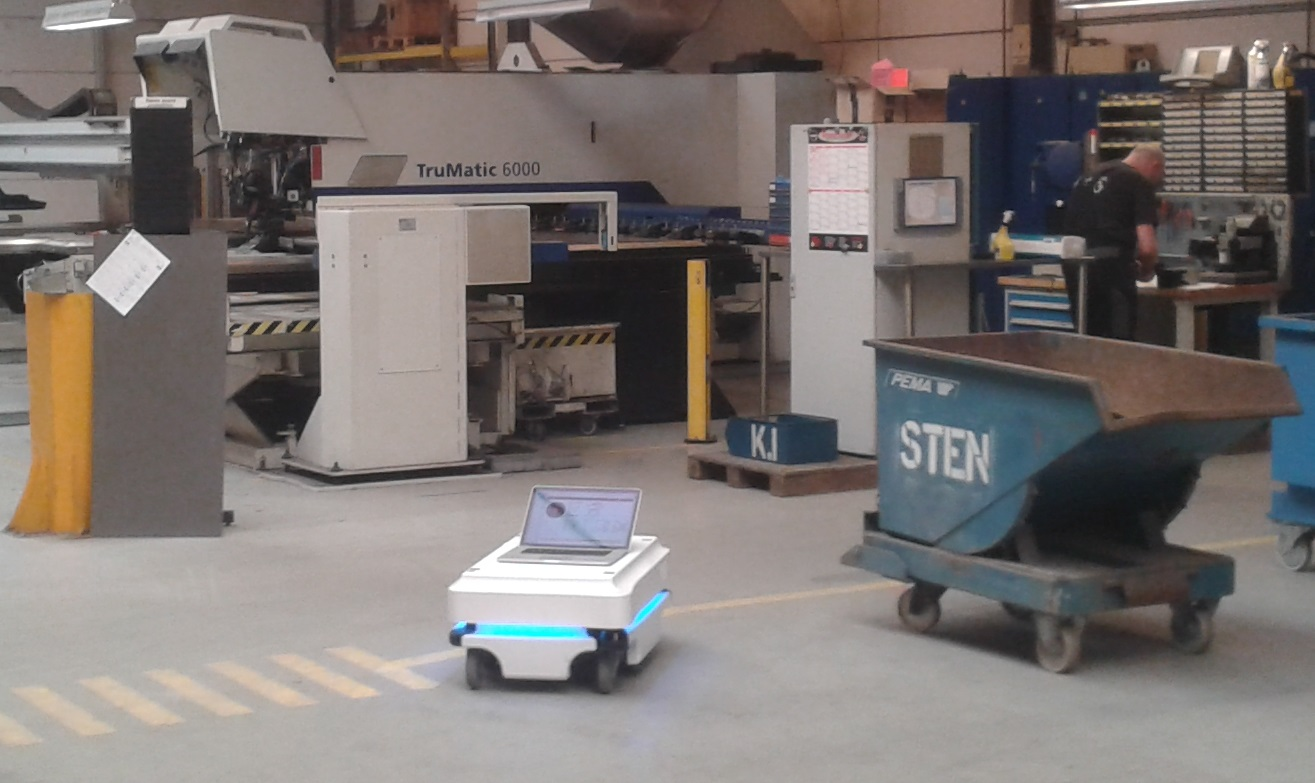
\includegraphics[width=1.0\textwidth]{chapters/mapping_of_dynamic_areas/figures/scan-mir}	
		\caption{MiR-100 robot navigating close to heavy machinery.}
		\label{fig:scan-mir}
	\end{subfigure}
	\begin{subfigure}[t]{0.3875\textwidth}
		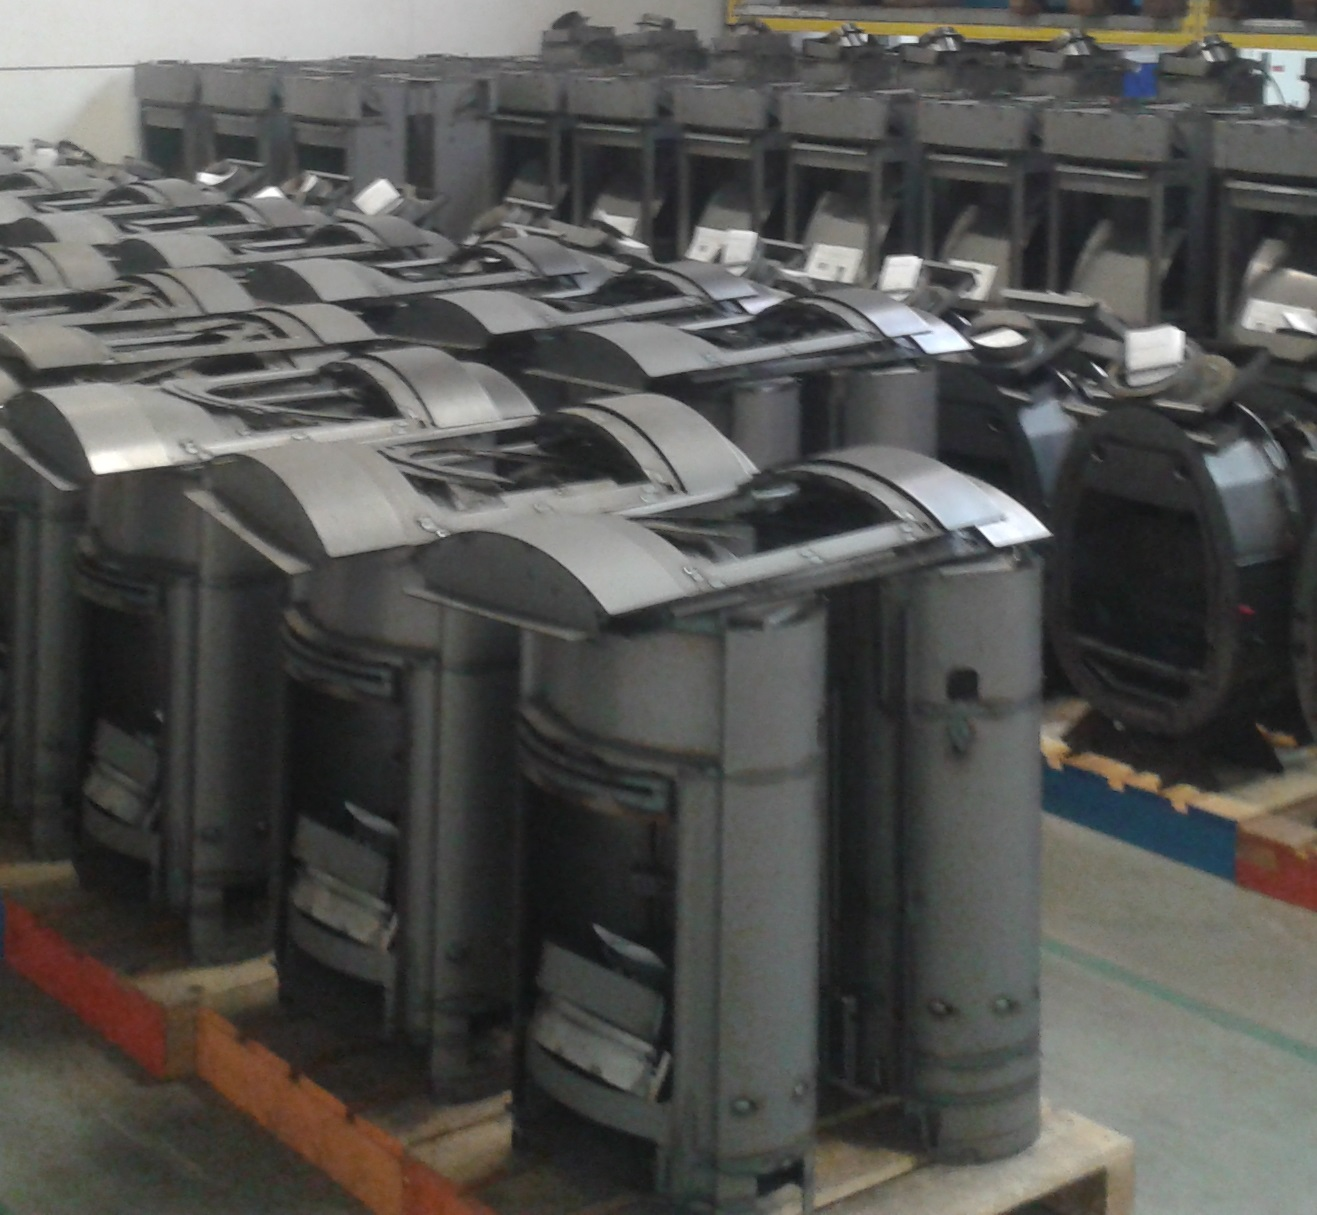
\includegraphics[width=1.0\textwidth]{chapters/mapping_of_dynamic_areas/figures/scan-semi-static-obstacles}
		\caption{\textit{Semi-static} obstacles in the form of product parts.}
		\label{fig:scan-semi-static-obstacles}
	\end{subfigure}
	\caption{Examples of obstacles in the production area at SCAN A/S.}
\end{figure}

The information of these areas can be incorporated into the representation of the world to avoid having to re-plan a path and improve localization. 

While navigating, \textit{highly dynamic} objects should not be considered as obstacles, but some re-planning of the path might be unavoidable due to them. 
It is beneficial to consider \textit{semi-static} obstacles in path planning to avoid having to re-plan, but by assigning them as lethal obstacles it might be impossible to plan a path although one might exist.
The \textit{static} objects should always be present as lethal obstacles when path planning to avoid navigating along obscure routes.

For localization, \textit{highly dynamic} objects should not be included as landmarks since they are moving almost constantly. 
Since the value of the \textit{semi-static} obstacles as landmarks depends on how dynamic they are, they should be weighted in the localization algorithm accordingly. 
The \textit{static} obstacles are very good landmarks.